% Compile with pdflatex. The editable figure is included below.
\documentclass[11pt,letterpaper]{article}
\usepackage[T1]{fontenc}
\usepackage[utf8]{inputenc}
\usepackage{lmodern,microtype,tikz,hyperref,fancyhdr}
\usepackage[margin=0.88in,headheight=14pt,headsep=12pt]{geometry}
\usepackage[compact]{titlesec}
\definecolor{ink}{HTML}{1C4448}
\definecolor{steel}{HTML}{CBDCDA}
\definecolor{accent}{HTML}{883948}
\hypersetup{colorlinks=true,urlcolor=ink,linkcolor=ink}
\titleformat{\section}{\sffamily\Large\bfseries\color{ink}}{}{0pt}{}
\titleformat{\subsection}{\sffamily\normalsize\bfseries\color{ink}}{}{0pt}{}
\setlength{\parindent}{0pt}
\setlength{\parskip}{0.54em}
\setlength{\emergencystretch}{1.5em}
\pagestyle{fancy}\fancyhf{}\lhead{\small\sffamily NSF AMDO}\rhead{\small\sffamily Provisional project description}\rfoot{\small\sffamily Collaborative working draft\quad\thepage}
\begin{document}

\section*{Stock Allocation Changes How a Milled Plate Bends}

A thin aluminum plate can meet its thickness specification under clamps and fail its flatness specification after release. While both faces still carry excess stock, the machinist can remove more from either face and leave the finished thickness unchanged. The choice determines which layers of metal remain. To see how the unfinished plate bends, the machinist can remove the clamps and measure its free shape. Doing so costs a setup and can change how the plate sits for the next cut.

\subsection*{Which plate warrants another setup?}

A released shape records the bending effect of stresses through the remaining thickness. Two plates can have the same bow while carrying stress at different depths. Cutting a layer from the same face can then drive one plate toward its drawing and the other away from it. We propose to learn when the known stock origin and cutting history resolve this ambiguity and when observing released shape changes the better allocation. The practical test is whether the resulting choice improves conformance enough to justify the interruption.

\begin{center}

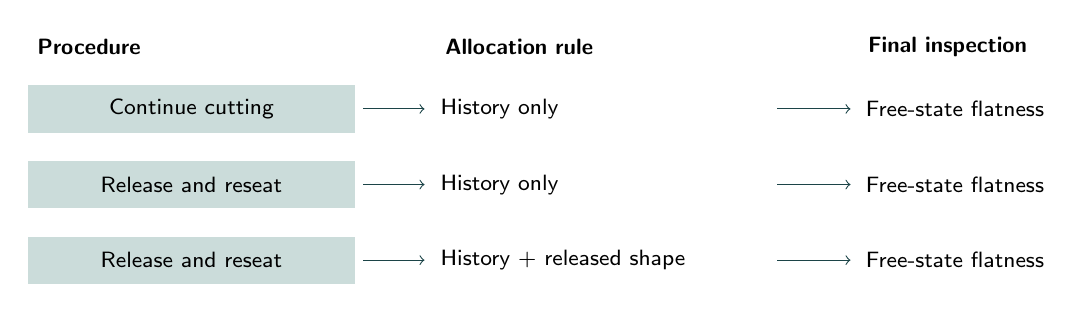
\begin{tikzpicture}[x=1cm,y=1cm,font=\sffamily\footnotesize,every node/.style={align=center}]
\node[anchor=west,font=\sffamily\bfseries\footnotesize] at (0,2.84){Procedure};
\node[anchor=west,font=\sffamily\bfseries\footnotesize] at (5.18,2.84){Allocation rule};
\node[anchor=west,font=\sffamily\bfseries\footnotesize] at (10.55,2.84){Final inspection};
\foreach \y/\procedure/\rule in {2.05/Continue cutting/History only,1.09/Release and reseat/History only,0.13/Release and reseat/History + released shape}{
  \fill[steel] (0,\y-.30) rectangle (4.16,\y+.30);
  \node at (2.08,\y){\procedure};
  \draw[->,ink] (4.26,\y)--(5.04,\y);
  \node[anchor=west] at (5.12,\y){\rule};
  \draw[->,ink] (9.52,\y)--(10.45,\y);
  \node[anchor=west] at (10.52,\y){Free-state flatness};
}
\end{tikzpicture}

\end{center}

{\small\textbf{Figure 1.} Both reseated arms receive the same scan. Revealing its result changes only the information available when selecting a face split. All three arms receive blinded final inspection.}

History-based adjustment of machining allowances has already been demonstrated on physical parts [1]. Remaining-stock limits establish when a shifted section can still meet its drawing [2]. An NSF GOALI award also coupled residual-stress estimation and tool-path design [4]. We will test whether the better allocation reverses among feasible parts, whether the reversal can be predicted on new stock, and how much the extra setup buys.

\newpage

\section*{Aim 1 · Test for reversals in the better finishing cut}

\textbf{Year 1.} Satish Bukkapatnam's group will qualify one functioning CNC mill, one two-sided fixture and an independent gauge for final free-state flatness. The drawing must permit a floating final mid-plane and leave enough stock for both faces to clean up under either split [2]. The group has demonstrated motion sensing on a Langmuir MR-1 [7], and Texas A\&M lists shared CNC equipment [5]. Qualification requires a staffed cut under load at the proposed dimensions, traceable stock, and repeated release, support and reseating trials. We will measure gauge scatter on repositioned parts, check the effect of temperature and supports, and time the setup on the occupied machine.

\subsection*{Cross the face split with recorded stock origin}

We will cut sibling blanks from neighboring mapped positions in independent parent plates. Mark the original face and rolling direction, record the through-thickness origin, and apply a common roughing cut within each stock level. Before finishing, measure the full released profile on repeatable supports. At each tested level retain two preregistered allocations with the same total removal and final thickness. Randomize individual blanks to those splits within parent, origin and stock-level blocks. Each blank supplies a final flatness and a signed curvature along the marked axis under one allocation. A treatment contrast requires several independently cut blanks in each arm.

We will test two complementary predictions. Among blanks with profiles alike within an equivalence band set from gauge repeatability, does stock origin and prior removal history predict that opposite splits work best? Within a common recorded history, do distinguishable profiles predict a reversal? The first test identifies what a shape-only rule misses. The second identifies a reason to buy the reading. A reversal requires the estimated split advantage to change sign across the prespecified groups by a shop-relevant margin. For example, one history must favor greater removal from the marked face and a second history must favor greater removal from the opposite face. The randomized response in each group distinguishes a reversal from one generally superior split.

\subsection*{First decision on experimental scale}

Bukkapatnam will deliver the cut records, timed reseats and uncertainty of the independent gauge to Rui Tuo and Xianyang Zhang. Zhang will estimate sibling and parent variation to determine how many parent plates can resolve a useful reversal. If the drawing prevents a second allocation, the measurement obscures that margin, or the required independent stock exceeds the available campaign, the full trial loses its experimental basis.

\newpage

\section*{Aim 2 · Identify which observations change the cut}

\textbf{Year 2.} Tuo will predict the difference in final flatness between the same two allocations at a specified stock level. One model propagates an inherited through-thickness stress profile as the two faces are removed. The other also allows the preceding cuts to alter stress in a shallow surface layer. Two candidate profiles can give indistinguishable relaxed shapes if their bending moments agree. Removing a slice changes both its share of that moment and the stiffness of what remains. This gives the models a physical opportunity to predict different responses on the next cut.

Using development plates, Tuo will specify pairs of stock histories that give similar prefinish shapes but opposite predicted signs for the split advantage. He will also identify histories in which an added shape reading moves the preferred split and histories in which it adds little. Bukkapatnam's group will machine new siblings for both splits in each test. Building on their model-validation work [6], Zhang will compare the signed, prespecified allocation contrasts with independent free-state measurements on fresh parent plates, including cases where the models agree. Selection for model disagreement alone would overstate the prevalence of useful readings.

\subsection*{Check the mechanical explanation independently}

Randomized cuts can establish which allocation performs better. Attribution to inherited or machining-induced stress requires an additional observation. Subject to qualification, sacrificial matched blanks will supply an separate bulk-stress estimate from incremental layer removal and surface-stress measurements after roughing by X-ray diffraction. On parent stock reserved for this test, we will compare measured signs, depths and uncertainty with predictions recorded before testing [3,8]. Both methods sample siblings, so a model that predicts the better allocation but misses the stress observations supports a decision rule only. If the reference measurements are unavailable, the stress-source attribution remains open.

\subsection*{Freeze what the operator can know}

We will compare the added reading with the best fixed split, an adapted history-based allowance rule [1], and a reduced-layer-removal predictor [3]. Each comparator will carry the cost of the equipment and observations it requires. Tuo and Zhang will freeze the stop rule using only stock origin, pre-interruption cutting records and available stock. It may recommend stopping in several stock ranges. They will also fix the history-only and reading-informed split rules, feasible actions, uncertainty margins, and the distribution of jobs over which to evaluate them. A reversal among unusual blanks may establish a physical effect yet yield little production benefit if those blanks seldom enter the shop.

\newpage

\section*{Aim 3 · Measure the return on one interruption}

\textbf{Year 3.} Reserve complete parent plates before model fitting. On each validation blank, log the frozen stop decision before releasing any clamp. Where the rule calls for a stop, randomize within parent and stock level to continuous machining, release/scan/reseat with the reading withheld, or the same procedure with the reading visible. The first two use the frozen history-only split. The third may use the new reading. Where the rule calls for continuing, follow that route and retain those blanks in the overall estimate. A blinded inspector will grade every released plate on the same supports after thermal equilibration.

Zhang will report drawing yield, absolute flatness error and occupied machine minutes. Visible versus withheld readings estimate the benefit of the data. Withheld versus continuous cutting estimates the effects of handling and delay. Visible versus continuous estimates the operational gain in the stop region. Weight that gain by the proportion of eligible jobs to evaluate the complete policy. Resample or model whole parent plates for uncertainty. Individual blanks are randomized units. Scans, locations and sibling blanks from a common parent cannot stand in for independent stock purchases.

\subsection*{What a shop can use}

The shop will receive a table keyed to remaining stock and recorded history. It will show when to continue machining and when to measure, which face should supply the larger cut under each reading, and where the evidence leaves the two splits equivalent or unresolved. The accompanying drawing and range of stock origins will define its scope. We will report additional machine minutes per reject avoided when yield improves, and convert that estimate to a break-even reject cost if the shop supplies an hourly rate. A teaching dataset will let machining students select a split before seeing independently graded outcomes. The three-year scientific case ends if a fixed or history-only split performs equivalently even in predicted reversal cases. A resolved reversal with no net economic gain would support the physical finding while favoring continued machining. Intervals spanning meaningful benefit and harm leave the decision unresolved.

\subsection*{Selected sources}

\begin{enumerate}
\small\setlength{\itemsep}{0pt}
\item \href{https://doi.org/10.1016/j.cja.2020.03.038}{Hao et al. Online deformation monitoring and machining allowance control.}
\item \href{https://doi.org/10.1016/j.cirp.2015.04.025}{Li et al. Stock allowance and compensation of machining distortion.}
\item \href{https://doi.org/10.3390/jmmp8010009}{Aurrekoetxea et al. Machining distortion prediction from reduced layer removal.}
\item \href{https://www.nsf.gov/awardsearch/showAward?AWD_ID=1762722}{NSF. GOALI machining distortion project, award 1762722.}
\item \href{https://texasmakes.tamu.edu/facilities/}{Texas A\&M. Institute for Manufacturing Systems facilities.}
\item \href{https://arxiv.org/abs/2604.17144}{Li, Zhang and Tuo. Physical model validation against observations. Preprint, 2026.}
\item \href{https://ssrn.com/abstract=7243783}{Hanchate et al. Machine-tool digital twin architecture and validation. Preprint, 2026.}
\item \href{https://doi.org/10.1007/s11340-021-00734-5}{Chighizola et al. Comparing near-surface stress measurements in milled aluminum.}
\end{enumerate}

\end{document}
